\documentclass[aspectratio=169]{beamer}

\usetheme{default}
\setbeamertemplate{navigation symbols}{}
\setbeamertemplate{footline}[frame number]
\usepackage[T1]{fontenc}
\usepackage[utf8]{inputenc}
\usepackage{lmodern}

\title{Concept Drift, Continuous ML, MLOps \& CCAM:\\
A Drift-aware Platform}
\author{Angelis Georgios, Kyriakopoulos Georgios, Tzelepis Serafeim}
\institute{School of Electrical and Computer Engineering, National Technical University of Athens}
\date{28 July 2025}

\begin{document}

\begin{frame}
  \titlepage
\end{frame}

\begin{frame}{Agenda}
  \tableofcontents
\end{frame}

%================================================
\section{1) Thesis Scope}
\begin{frame}{Thesis Scope}
  \begin{itemize}
    \item Build a \textbf{drift-aware platform} for mobility models on Athens center.
    \item Generate \textbf{synthetic traffic data} from SUMO (Simulation of Urban MObility).
    \item \textbf{Three regression tasks}: ETA, Fuel Consumption, Number of Stops.
    \item Show end-to-end: \textbf{stable} $\rightarrow$ \textbf{drift} $\rightarrow$ \textbf{detect} $\rightarrow$ \textbf{retrain} $\rightarrow$ \textbf{mitigate}.
    \item Deliverables: dataset generation pipeline, tuned models for each task, platform (backend, frontend, drift service, model services).
  \end{itemize}
\end{frame}

%================================================
\section{2) Problem Statement}
\begin{frame}{Concept Drift \& Why It Matters}
  \begin{itemize}
    \item \textbf{What it is:} When the real world changes, the link between inputs and the target also changes over time (non-stationarity).
    \item \textbf{Why it happens:} Seasons and trends, one-off events, policy or product changes, and even sensor or software updates.
    \item \textbf{Why it matters:} If we don't watch for it, model accuracy quietly drops, dashboards stop matching reality, and decisions become costly or unsafe.
    \item \textbf{What to do:} Treat ML as a live system—\textbf{monitor} data and outcomes, \textbf{detect} changes early, and \textbf{adapt}.
  \end{itemize}
\end{frame}

\begin{frame}{Our ML Tasks}
  \begin{itemize}
    \item \textbf{Estimated Time of Arrival (ETA)}: essential for accurate route planning and improving user satisfaction.
    \item \textbf{Fuel Consumption}: key to reducing operating costs and CO$_2$ emissions via eco-routing.
    \item \textbf{Number of Stops}: influences perceived trip quality and helps optimize overall traffic flow.
  \end{itemize}
\end{frame}

%================================================
\section{3) Software Design \& Tools}
\begin{frame}{Software Design \& Tools}
  \begin{itemize}
    \item \textbf{Synthetic Data}: SUMO - Python.
    \item \textbf{Models}: XGBoost/LightGBM/CatBoost, scikit-learn, numpy, pandas - Python.
    \item \textbf{Backend}: FastAPI - Python.
    \item \textbf{Drift}: River (ADWIN, KSWIN, PageHinkley) - Python.
    \item \textbf{UI}: Dash/Plotly - Python.
    \item \textbf{Data}: Parquet/CSV files.
    \item \textbf{Orchestration}: Docker.
  \end{itemize}
\end{frame}

%================================================
\section{4) Data Acquisition}
\begin{frame}{Athens Network Configurations \& Traffic Patterns}
  \begin{itemize}
    \item \textbf{Base network}: SUMO network built from OSM data over central Athens.
    \item \textbf{Rain network}: same map area, but with friction reduced in all lanes (1.0 $\rightarrow$ 0.4) to simulate wet conditions.
    \item \textbf{Traffic generation periods}: per-hour volumes with morning and afternoon peaks, and lower mid-day activity.
    \item \textbf{Realistic variability}: added random noise to hourly volumes and used a distinct random seed for each 10h day simulation.
  \end{itemize}
\end{frame}

\begin{frame}{Dataset Structure}
  \begin{itemize}
    \item \textbf{Three CSV files} (each $\sim$55--60\,k trips over a 10 hour simulation):
      \begin{itemize}
        \item \texttt{train-fcd.csv} \quad (base network)
        \item \texttt{test-fcd.csv}  \quad (base network)
        \item \texttt{rain-fcd.csv}  \quad (rain-modified network)
      \end{itemize}
    \item \textbf{Columns (per row)}:
      \texttt{timestep, vehicle\_id, x, y, speed, lane, odometer, fuel, waiting\_time}
  \end{itemize}
\end{frame}

\begin{frame}{Dataset Generation Pipeline}
  \begin{itemize}
    \item \textbf{osmGet}: extract OSM data within a bounding box over central Athens
    \item \textbf{osmBuild}: convert OSM into a SUMO-compatible network file
    \item \textbf{randomTrips}: generate vehicle trips using per-hour traffic volumes and a different random seed
    \item \textbf{sumo}: run 10-hour simulations, export Floating Car Data (FCD) and emission logs
  \end{itemize}
\end{frame}

%================================================
\section{5) Implementation}
\begin{frame}{Data Preprocessing \& Feature Engineering}
  \begin{itemize}
    \item \textbf{Trip extraction}: group raw FCD by vehicle into one row per trip (origin-destination)
    \item \textbf{Different features} added per model:
      \begin{itemize}
        \item \emph{Temporal}: \texttt{hour\_bin}
        \item \emph{Spatial}: source/destination clusters (\texttt{x,y})
        \item \emph{Route}: number of edges traversed, distance measures (Euclidean, Manhattan, Haversine)
      \end{itemize}
    \item \textbf{Result}: tabular dataset with inputs + ground-truth targets (ETA, fuel, stops)
  \end{itemize}
\end{frame}

\begin{frame}{Model Training \& Evaluation}
  \begin{itemize}
    \item \textbf{Evaluation metrics}:
    \begin{itemize}
      \item \emph{Primary}: MAE
      \item \emph{Secondary}: MAPE, \(R^2\), RMSE, MSE
    \end{itemize}
    \item \textbf{Hyperparameter tuning}: Optuna / grid search over
    \texttt{n\_estimators}, \texttt{max\_depth}, \texttt{learning\_rate}, \texttt{subsample}, …
    \item \textbf{Outcome}: XGBoost delivered the best trade-off of accuracy and training speed for all three tasks
  \end{itemize}
\end{frame}

\begin{frame}{High-level Architecture}
\begin{itemize}
  \item \textbf{Frontend (Dash/Plotly)}: Admin tab (live MAE charts, notifications, run controls); User tab (Athens map, O/D query).
  \item \textbf{Orchestrator (FastAPI)}: simulation clock, batch prediction, error calc, drift ensemble, per-model state, UI feed, controls.
  \item \textbf{Model Service (FastAPI)}: per-task pipelines (preprocessing + booster), \texttt{/predict}, \texttt{/retrain}, \texttt{/load}.
  \item \textbf{Filesystem Store}: Parquet datasets (\texttt{train/test/rain}); filesystem model registry (\texttt{models/\{task\}/vN/}).
  \item \textbf{Docker Compose}: orchestration with multiple containers.
\end{itemize}
\end{frame}

\begin{frame}{Components Diagram}
  \begin{center}
    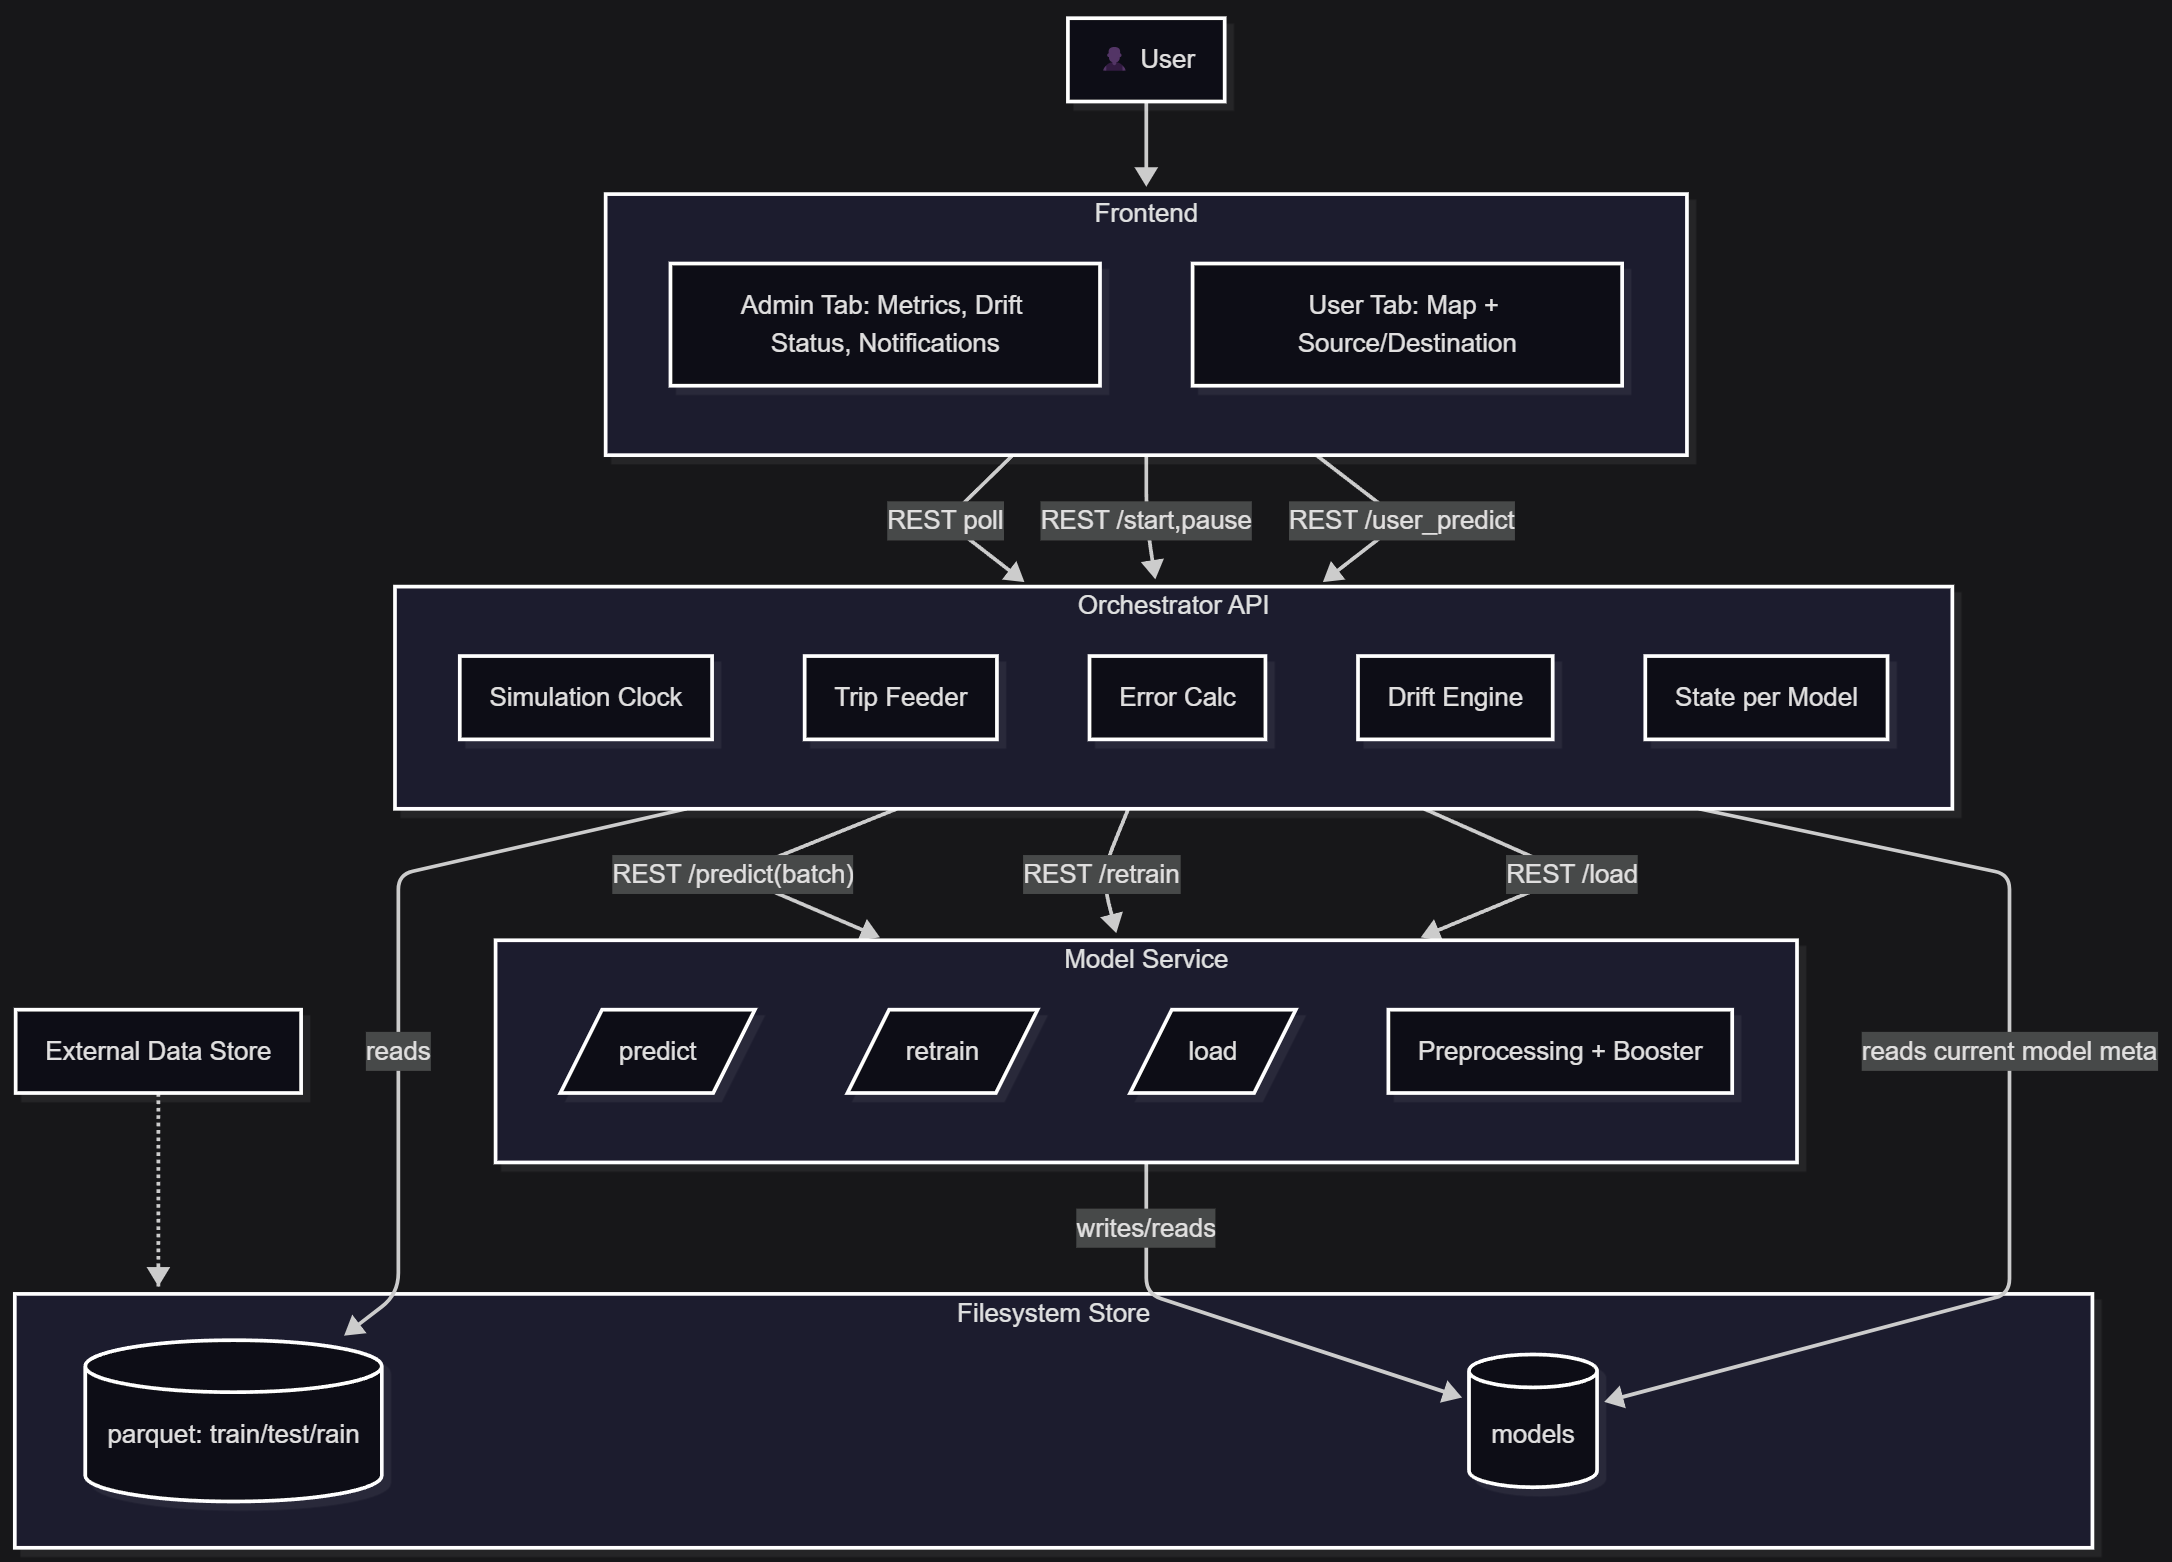
\includegraphics[height=0.85\textheight,keepaspectratio]{figures/components-diagram.png}
  \end{center}
\end{frame}

%================================================
\section{6) Platform Overview}
\begin{frame}{How It Works (at a glance)}
\begin{enumerate}
  \item \textbf{Timelapse clock}: compress 20\,h of trips (test then rain) into a few minutes.
  \item \textbf{Per tick}: Orchestrator pulls trips whose \texttt{sim\_time} falls in the current window.
  \item \textbf{Batch predict}: send features to Model Service; receive predictions for ETA/Fuel/Stops.
  \item \textbf{Immediate ground truth}: join with labels; compute per-trip absolute errors.
  \item \textbf{Live metrics}: update rolling MAE per task and push to the UI feed.
  \item \textbf{Drift monitoring}: feed a smoothed error stream into ADWIN, Page--Hinkley, KSWIN, and an SPC rule; raise drift on majority vote.
  \item \textbf{Mitigation}: after drift is confirmed, collect N more “rain” trips, trigger retraining, then swap to the new model version.
  \item \textbf{Repeat per model}: ETA, Fuel, Stops progress through the same state machine independently.
\end{enumerate}
\end{frame}

\begin{frame}{Admin Tab: Sped-up Simulation \& Drift Story}
\begin{itemize}
  \item \textbf{Three live charts} (ETA/Fuel/Stops): rolling MAE; drift state (Stable/Confirmed/Collecting/Retraining/Swapped).
  \item \textbf{Notifications}: day transition at 10\,h (\emph{rain starts}), drift detected (\emph{votes \(\ge\)3}), retrain started/completed, model swapped to v\(N\).
  \item \textbf{What you see}: errors rise after rain; drift fires; we keep predicting with old model while “collecting” rain data; retrain runs; swap reduces error (not all the way to baseline).
  \item \textbf{Controls}: Start/Pause/Resume/Restart.
\end{itemize}
\end{frame}

\begin{frame}{Admin Tab: Sped-up Simulation \& Drift Story}
  \begin{center}
    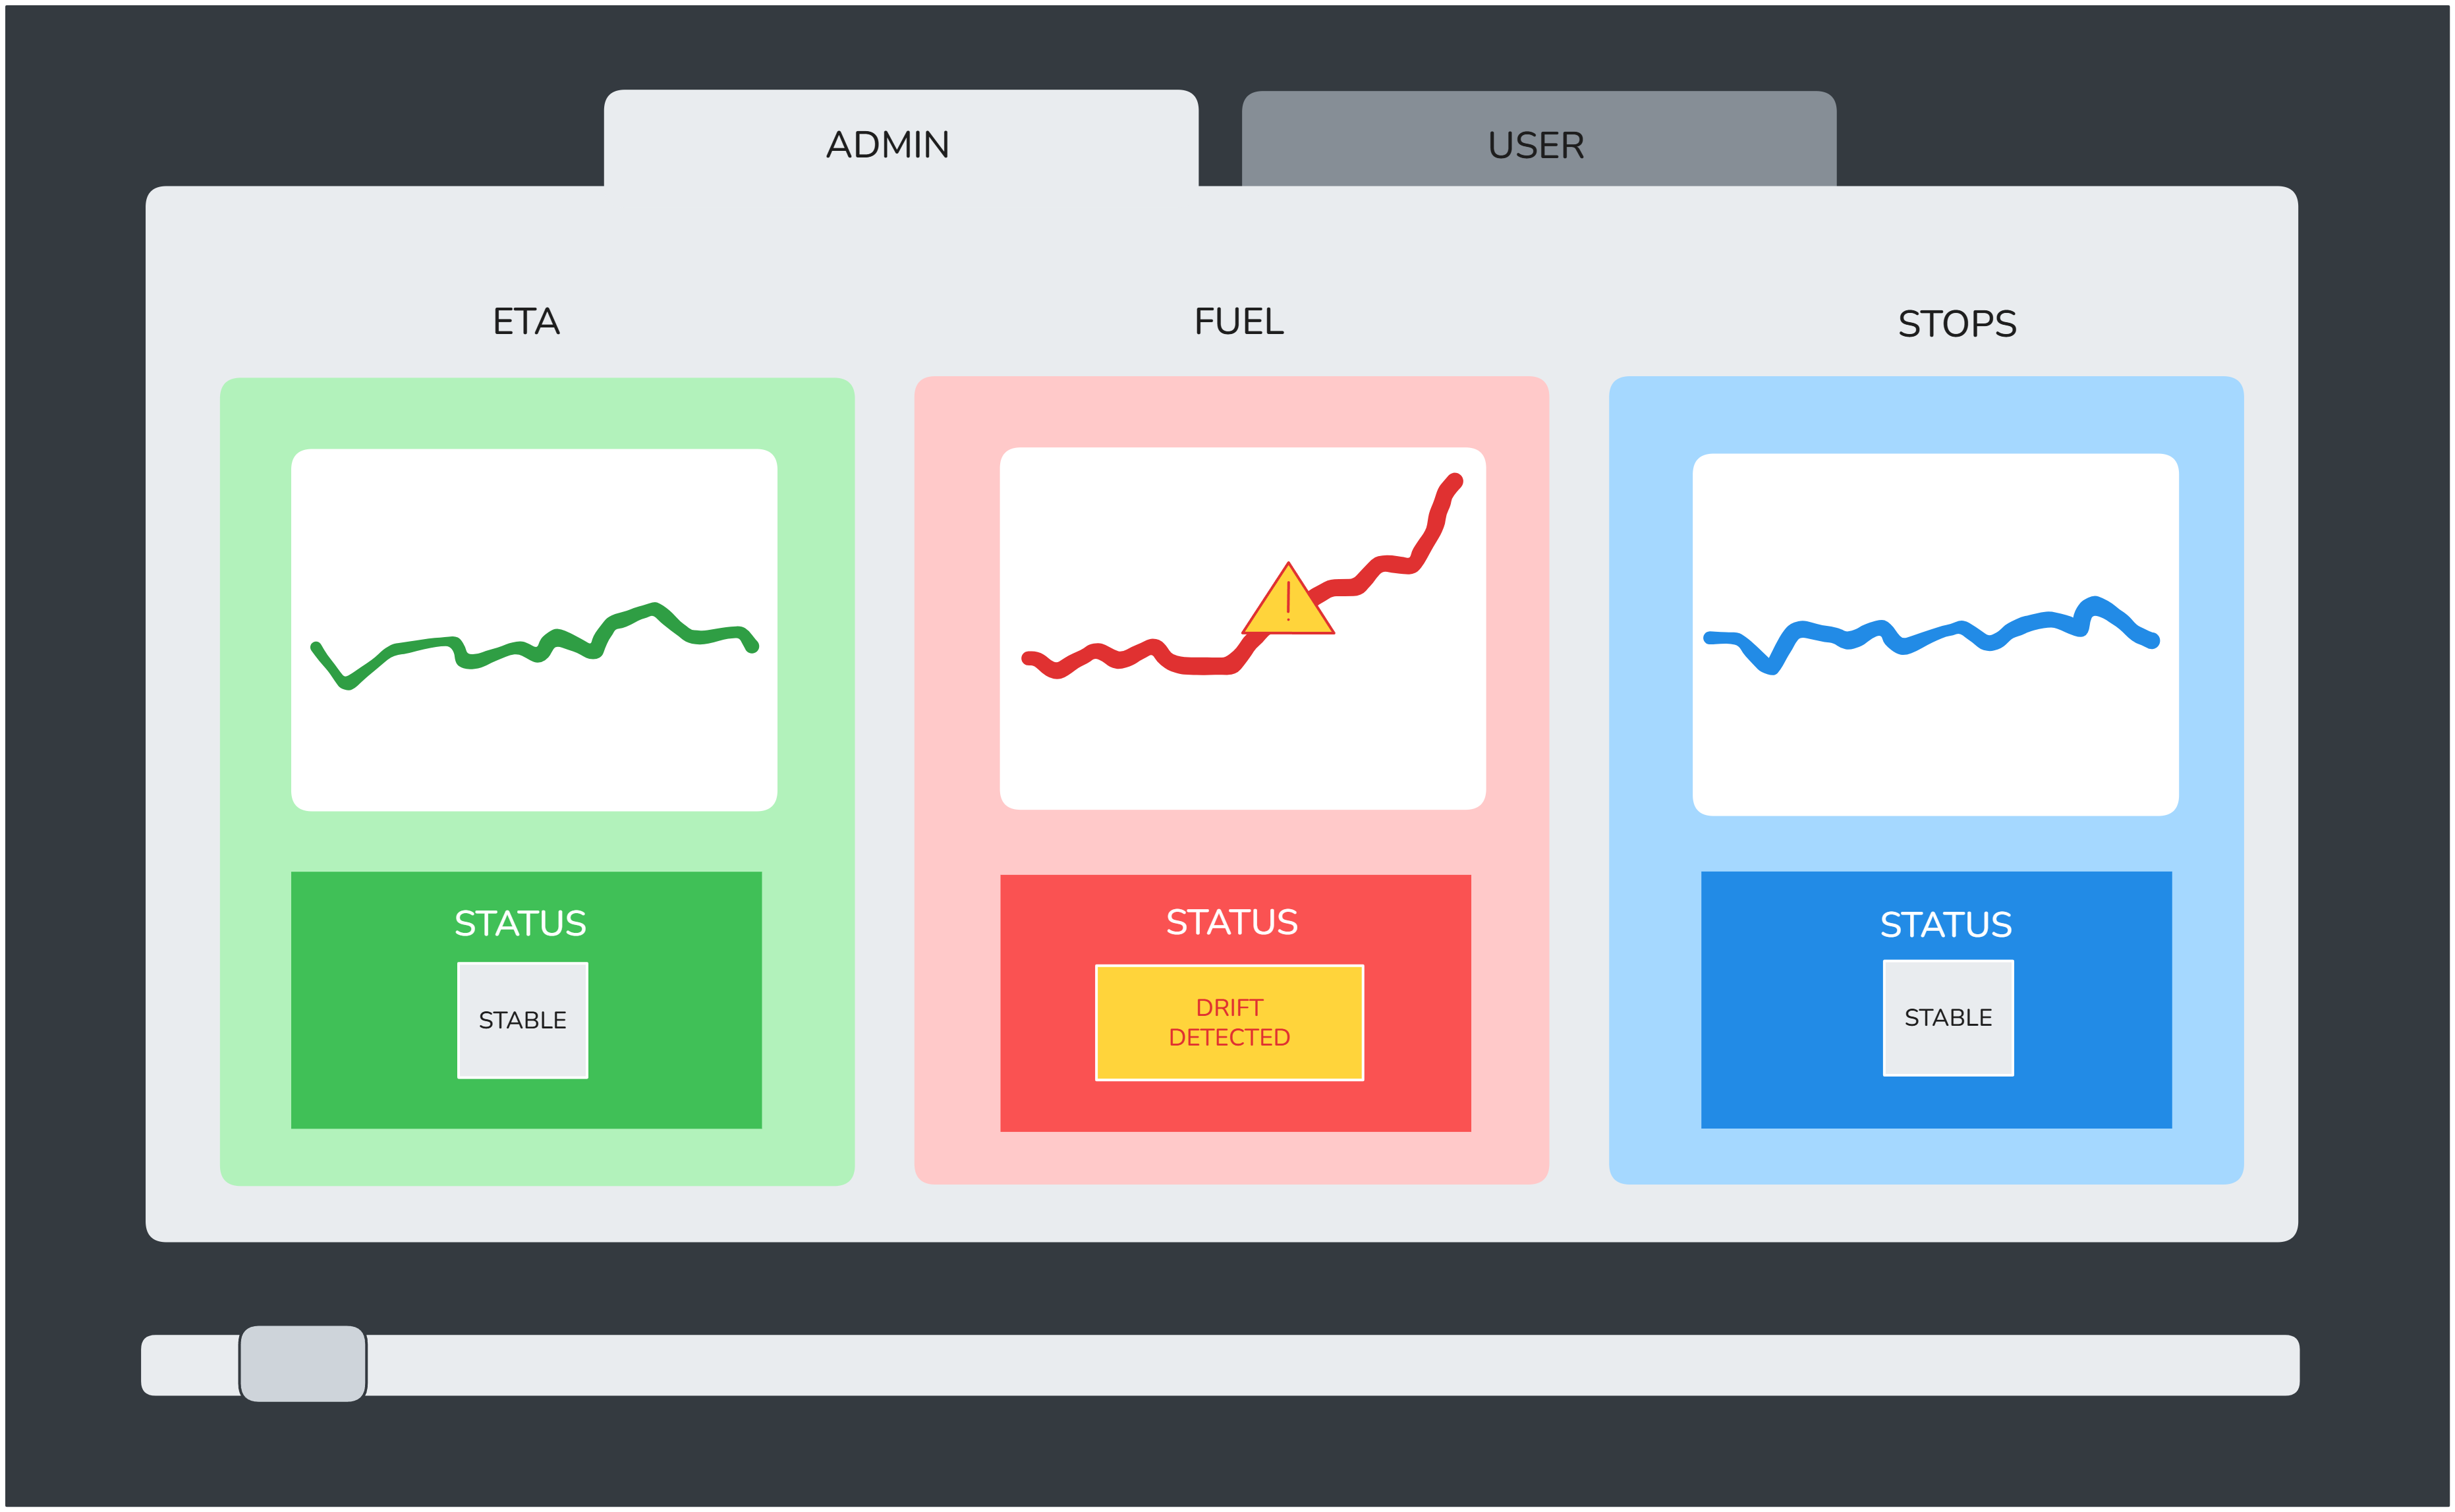
\includegraphics[height=0.85\textheight,keepaspectratio]{figures/admin-tab.png}
  \end{center}
\end{frame}

\begin{frame}{User Tab: Predictions at the Current State}
\begin{itemize}
  \item \textbf{Map of central Athens}: user picks \textbf{source} and \textbf{destination}.
  \item \textbf{Uses the same simulation time}: features derive from current \texttt{sim\_time} (e.g., \texttt{hour\_bin}, distance, spatial bins).
  \item \textbf{Calls active models}: returns ETA, Fuel, Stops from whichever version is currently loaded (pre‑ or post‑swap).
  \item \textbf{Consistent context}: shows badges like “Rain scenario” and current drift state so predictions match what the Admin tab shows.
  \item \textbf{Demo behavior}: \emph{pauses} the timelapse while in the User tab, then \emph{resumes} when you go back to Admin.
\end{itemize}
\end{frame}


\begin{frame}{User Tab: Predictions at the Current State}
  \begin{center}
    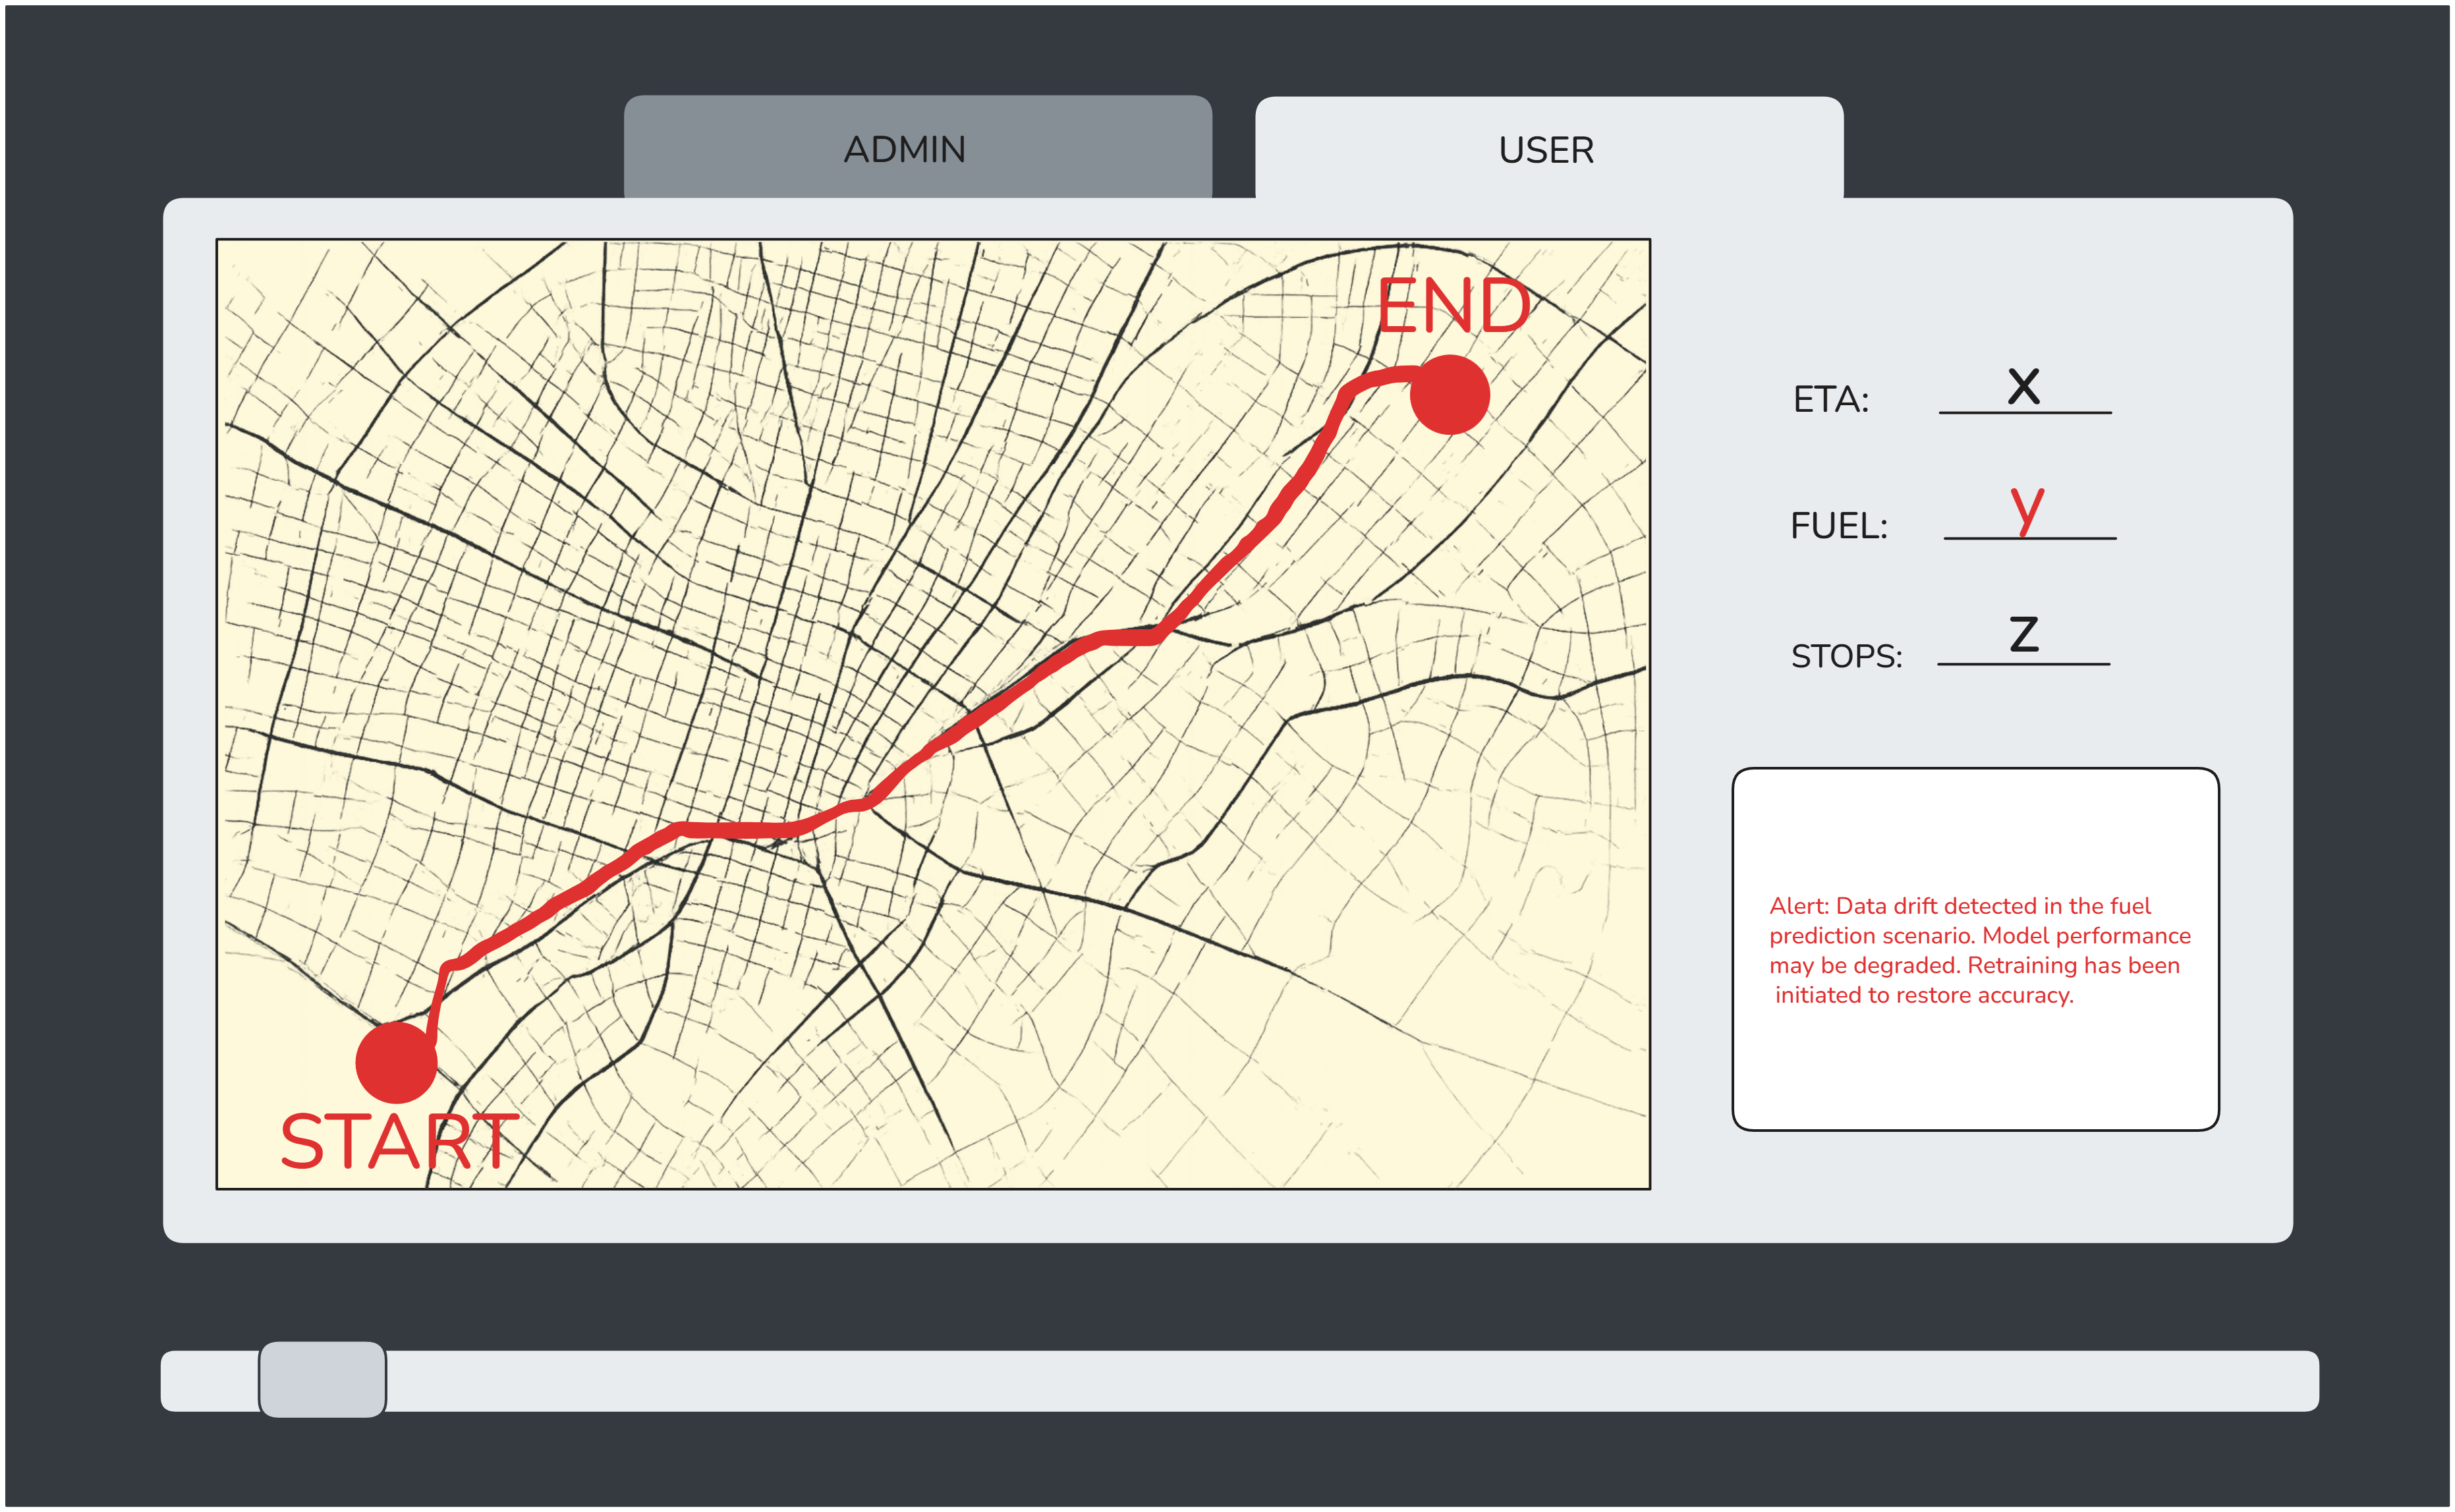
\includegraphics[height=0.85\textheight,keepaspectratio]{figures/user-tab.png}
  \end{center}
\end{frame}

%================================================
\section{7) Implementation Challenges}
\begin{frame}{Implementation Challenges}
\begin{itemize}
  \item \textbf{Road closures drift scenario:} Closing lanes/edges to mimic events/roadworks in SUMO led to unstable routing and distorted traffic patterns. We therefore used the rain/friction shift as a controlled, repeatable drift.
  \item \textbf{Parking availability task:} The current SUMO setup lacks realistic parking supply/occupancy and consistent stop events, so the task could not be integrated or evaluated alongside the trip-level models.
  \item \textbf{Time-series traffic speed model:} A lagged-input traffic speed model adapted quickly to the rain shift and showed little error increase, making drift hard to showcase; we replaced it with the “number of stops” task which reacts clearly.
\end{itemize}
\end{frame}

\begin{frame}{Questions}
  \centering \Large Thank you!
\end{frame}

\end{document}
